% tikzpicture starts at line 1488 of input.tex
\documentclass{standalone}

\usepackage{amsthm, amsmath}

% Prevent the eventual "Too many alphabets" error
\newcommand\hmmax{0}
\newcommand\bmmax{0}

\RequirePackage{notomath}
\RequirePackage{inter}
\RequirePackage[scaled=0.85]{DejaVuSansMono}
\def\bfseries@rm{sb}

\DeclareMathVersion{sansmath}
\SetSymbolFont{operators}{sansmath}{OT1}{NotoSans-TLF}{m}{n}
\SetSymbolFont{letters}{sansmath}{OML}{notosansmi}{m}{it}
\SetMathAlphabet\mathbf{sansmath}{OT1}{NotoSans-TLF}{b}{n}
\SetMathAlphabet\mathsf{sansmath}{OT1}{NotoSans-TLF}{m}{n}
\SetMathAlphabet\mathit{sansmath}{OT1}{NotoSans-TLF}{m}{it}

\DeclareMathVersion{sansmathbold}
\SetSymbolFont{operators}{sansmathbold}{OT1}{NotoSans-TLF}{b}{n}
\SetSymbolFont{letters}{sansmathbold}{OML}{notosansmi}{b}{it}
\SetSymbolFont{symbols}{sansmathbold}{LMS}{ntxsy}{b}{n}
\SetMathAlphabet\mathbf{sansmathbold}{OT1}{NotoSans-TLF}{b}{n}
\SetMathAlphabet\mathsf{sansmathbold}{OT1}{NotoSans-TLF}{b}{n}
\SetMathAlphabet\mathit{sansmathbold}{OT1}{NotoSans-TLF}{b}{it}


% Upright Greek letters uppercase
\DeclareMathSymbol{\Gamma}{\mathord}{operators}{0}
\DeclareMathSymbol{\Delta}{\mathord}{operators}{1}
\DeclareMathSymbol{\Theta}{\mathord}{operators}{2}
\DeclareMathSymbol{\Lambda}{\mathord}{operators}{3}
\DeclareMathSymbol{\Xi}{\mathord}{operators}{4}
\DeclareMathSymbol{\Pi}{\mathord}{operators}{5}
\DeclareMathSymbol{\Sigma}{\mathord}{operators}{6}
\DeclareMathSymbol{\Upsilon}{\mathord}{operators}{7}
\DeclareMathSymbol{\Phi}{\mathord}{operators}{8}
\DeclareMathSymbol{\Psi}{\mathord}{operators}{9}
\DeclareMathSymbol{\Omega}{\mathord}{operators}{10}

% Italic Greek letters lowercase
\DeclareMathSymbol{\alpha}{\mathord}{letters}{11}
\DeclareMathSymbol{\beta}{\mathord}{letters}{12}
\DeclareMathSymbol{\gamma}{\mathord}{letters}{13}
\DeclareMathSymbol{\delta}{\mathord}{letters}{14}
\DeclareMathSymbol{\epsilon}{\mathord}{letters}{15}
\DeclareMathSymbol{\zeta}{\mathord}{letters}{16}
\DeclareMathSymbol{\eta}{\mathord}{letters}{17}
\DeclareMathSymbol{\theta}{\mathord}{letters}{18}
\DeclareMathSymbol{\iota}{\mathord}{letters}{19}
\DeclareMathSymbol{\kappa}{\mathord}{letters}{20}
\DeclareMathSymbol{\lambda}{\mathord}{letters}{21}
\DeclareMathSymbol{\mu}{\mathord}{letters}{22}
\DeclareMathSymbol{\nu}{\mathord}{letters}{23}
\DeclareMathSymbol{\xi}{\mathord}{letters}{24}
\DeclareMathSymbol{\pi}{\mathord}{letters}{25}
\DeclareMathSymbol{\rho}{\mathord}{letters}{26}
\DeclareMathSymbol{\sigma}{\mathord}{letters}{27}
\DeclareMathSymbol{\tau}{\mathord}{letters}{28}
\DeclareMathSymbol{\upsilon}{\mathord}{letters}{29}
\DeclareMathSymbol{\phi}{\mathord}{letters}{30}
\DeclareMathSymbol{\chi}{\mathord}{letters}{31}
\DeclareMathSymbol{\psi}{\mathord}{letters}{32}
\DeclareMathSymbol{\omega}{\mathord}{letters}{33}
\DeclareMathSymbol{\varepsilon}{\mathord}{letters}{34}
\DeclareMathSymbol{\vartheta}{\mathord}{letters}{35}
\DeclareMathSymbol{\varpi}{\mathord}{letters}{36}
\DeclareMathSymbol{\varrho}{\mathord}{letters}{37}
\DeclareMathSymbol{\varsigma}{\mathord}{letters}{38}
\DeclareMathSymbol{\varphi}{\mathord}{letters}{39}

% Change font tracking
\RequirePackage[letterspace=150]{microtype}

% Page breaking
\widowpenalty=10000
\clubpenalty=10000

%%%% Author's definition can start here

\usepackage{tikz}
\usepackage{tkz-graph}
\usepackage{mathdots}
\usepackage{dsfont}
\usetikzlibrary{shapes}

\DeclareMathOperator{\spn}{span}
\DeclareMathOperator{\tr}{tr}
\DeclareMathOperator{\rr}{\mathbb{R}}
\DeclareMathOperator{\cc}{\mathbb{C}}
\DeclareMathOperator{\arity}{arity}
\DeclareMathOperator{\vk}{\mathbf{K}}
\DeclareMathOperator{\vl}{\mathbf{L}}
\DeclareMathOperator{\vg}{\mathbf{G}}
\DeclareMathOperator{\vx}{\mathbf{x}}
\DeclareMathOperator{\vy}{\mathbf{y}}
\DeclareMathOperator{\vz}{\mathbf{z}}
\DeclareMathOperator{\va}{\mathbf{a}}
\DeclareMathOperator{\vb}{\mathbf{b}}
\DeclareMathOperator{\vq}{\mathbf{Q}}
\DeclareMathOperator{\vr}{\mathbf{R}}
\DeclareMathOperator{\vrr}{\mathbf{r}}
\DeclareMathOperator{\vc}{\mathbf{C}}
\DeclareMathOperator{\vcc}{\mathbf{c}}
\DeclareMathOperator{\vj}{\mathbf{J}}
\DeclareMathOperator{\vjj}{\mathbf{j}}
\DeclareMathOperator{\ic}{\mathcal{I}}
\DeclareMathOperator{\fc}{\mathcal{F}}
\DeclareMathOperator{\gc}{\mathcal{G}}
\DeclareMathOperator{\gk}{\mathfrak{G}_{\mathcal{F}}}
\DeclareMathOperator{\qk}{\mathfrak{Q}_{\mathcal{F}}}
\DeclareMathOperator{\stab}{Stab}
\newcommand{\tcwd}[1]{\left\langle #1 \right\rangle_{+, \circ, \otimes ,\top}}
\newcommand{\tcwdn}[1]{\left\langle #1 \right\rangle_{\circ, \otimes ,\top}}
\DeclareMathOperator{\holant}{Holant}
\DeclareMathOperator{\plholant}{Pl-Holant}
\DeclareMathOperator{\csp}{\#CSP}
\DeclareMathOperator{\qut}{Qut}
\DeclareMathOperator{\aut}{Aut}
\DeclareMathOperator{\eq}{\mathcal{EQ}}
\DeclareMathOperator{\geneq}{\mathcal{GEQ}}

\renewcommand*{\VertexSmallMinSize}{6pt}
% draw edges with diamonds in tikz
\newcommand{\DEdge}[2]{
    \draw[thick] (#1) -- (#2) node[draw, fill=white, kite, kite vertex angles = 120, minimum size = 4pt, inner sep = 1pt, pos=0.3, sloped] {};
}


\begin{document}
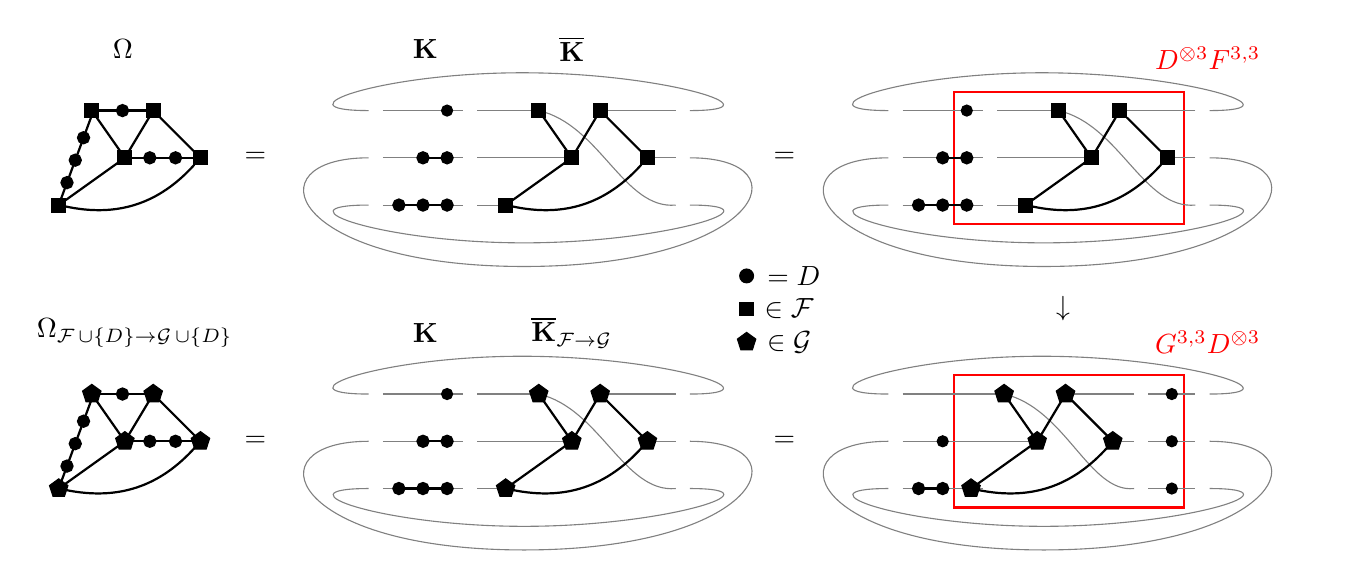
\begin{tikzpicture}[scale=0.6]
    \GraphInit[vstyle=Classic]
    \SetUpEdge[style=-]
    \SetVertexMath
    \tikzset{VertexStyle/.style = {shape=rectangle, fill=black, minimum size=5pt, inner sep=1pt, draw}}

    % length of dangling edges
    \def\dlen{1.7}
    \def\wlen{0.6}
    \def\wgap{0.3}
    \def\xsh{11}
    \def\ysh{-6}
    % x shift on G gadget in bottom left panel
    \def\ssh{-1.15}

    \def\labely{3.3}
    \node at (2.9,\labely) {$\Omega$};
    \node at (\xsh-1.7,\labely) {$\vk$};
    \node at (\xsh+1.4,\labely) {$\overline{\vk}$};
    \node at (3.15,\labely+\ysh) {$\Omega_{\fc\cup \{D\} \to \gc\cup \{D\}}$};
    \node at (\xsh-1.7,\labely+\ysh) {$\vk$};
    \node at (\xsh+1.4,\labely+\ysh) {$\overline{\vk}_{\fc\to\gc}$};

    \node at (\xsh-5.3,1) {$=$};
    \node at (\xsh-5.3,1+\ysh) {$=$};
    \node at (2*\xsh-5.1,1) {$=$};
    \node at (2*\xsh-5.1,1+\ysh) {$=$};

    \node at (2*\xsh+0.8,0.8+\ysh/2) {$\downarrow$};

    \node[draw, fill=black, circle, minimum size = 5pt, inner sep = 1pt] at (2*\xsh-5.9,1.5+\ysh/2) {};
    \node[draw, fill=black, regular polygon, regular polygon sides=4, minimum size = 7pt, inner sep = 1pt] at (2*\xsh-5.9,0.8+\ysh/2) {};
    \node[draw, fill=black, regular polygon, regular polygon sides=5, minimum size = 7pt, inner sep = 1pt] at (2*\xsh-5.9,0.1+\ysh/2) {};
    \node at (2*\xsh-4.9,1.5+\ysh/2) {$= D$};
    \node at (2*\xsh-5,0.8+\ysh/2) {$\in \fc$};
    \node at (2*\xsh-5,0.1+\ysh/2) {$\in \gc$};

    \node at (2*\xsh+3+0.6*\wlen+0.5,3.1) {$\textcolor{red}{D^{\otimes 3}F^{3,3}}$};
    \node at (2*\xsh+3+0.6*\wlen+0.5,3.1+\ysh) {$\textcolor{red}{G^{3,3}D^{\otimes 3}}$};
    % \Omega and boxes ================================================================================
    \foreach \y in {0,\ysh} {
    \begin{scope}[xshift=0.14*\xsh cm, yshift=\y cm]
        \draw[thick] (2,2) -- (0.7,2) 
            node[draw, fill=black, circle, minimum size = 4pt, inner sep = 1pt, pos=0.5] {};
        \draw[thick] (3,1) -- (1.4,1) 
            node[draw, fill=black, circle, minimum size = 4pt, inner sep = 1pt, pos=0.33] {}
            node[draw, fill=black, circle, minimum size = 4pt, inner sep = 1pt, pos=0.67] {};
        \draw[thick] (0,0) -- (0.7,1.9) 
            node[draw, fill=black, circle, minimum size = 4pt, inner sep = 1pt, pos=0.25] {}
            node[draw, fill=black, circle, minimum size = 4pt, inner sep = 1pt, pos=0.5] {}
            node[draw, fill=black, circle, minimum size = 4pt, inner sep = 1pt, pos=0.75] {};
    \end{scope}
    }

    \draw[color=red,thick] (2*\xsh-\wlen-\wgap-0.36*\dlen,2.4) rectangle (2*\xsh+3+0.6*\wlen,-0.4);
    \draw[color=red,thick] (2*\xsh-\wlen-\wgap-0.36*\dlen,2.4+\ysh) rectangle (2*\xsh+3+0.6*\wlen,-0.4+\ysh);

    % Extracted Omegas =========================================================================
    \foreach \x/\y in {0/0,\xsh/0,0/\ysh,\xsh/\ysh} {
    % Wraparound dangling edges
    \begin{scope}[xshift=\x cm, yshift=\y cm]
        % top
        \draw[thin, color=gray] 
        (\xsh-\dlen-\wlen-2*\wgap,2) .. controls 
        +(-2,0) and +(-3,0) ..
        (\xsh+0.35,2.8) .. controls
        +(3,0) and +(2,0) ..
        (\xsh+3+\wlen+\wgap,2);

        % inner bottom
        \draw[thin, color=gray] 
        (\xsh-\dlen-\wlen-2*\wgap,0) .. controls 
        +(-2,0) and +(-3,0) ..
        (\xsh+0.39,-0.8) .. controls
        +(3,0) and +(2,0) ..
        (\xsh+3+\wlen+\wgap,0);

        % outer bottom
        \draw[thin, color=gray]
        (\xsh-\dlen-\wlen-2*\wgap,1) .. controls
        +(-2.5,0) and +(-5,0) ..
        (\xsh+0.39,-1.3) .. controls
        +(5,0) and +(2.5,0) ..
        (\xsh+3+\wlen+\wgap,1);
    \end{scope}
    }

    \foreach \x/\y in {0/0,\xsh/0,0/\ysh} {
    % gadgets with all D on left
    \begin{scope}[xshift=\x cm, yshift=\y cm]
        \draw[thin, color=gray] (\xsh-\wlen,0) -- (\xsh,0);
        \draw[thin, color=gray] (\xsh-\wlen,2) -- (\xsh+0.7,2);
        \draw[thin, color=gray] (\xsh-\wlen,1) -- (\xsh+1.4,1);

        \draw[thin, color=gray] (\xsh+3+\wlen,0) .. controls (\xsh+2.5,-0.1) and (\xsh+2,1.7) .. (\xsh+0.7,2);
        \draw[thin, color=gray] (\xsh+3+\wlen,1) -- (\xsh+3,1);
        \draw[thin, color=gray] (\xsh+3+\wlen,2) -- (\xsh+2,2);
        \draw[thin, color=gray] (\xsh-\dlen-\wlen-\wgap,0) -- (\xsh-\wlen-\wgap,0);
        \draw[thin, color=gray] (\xsh-\dlen-\wlen-\wgap,1) -- (\xsh-\wlen-\wgap,1);
        \draw[thin, color=gray] (\xsh-\dlen-\wlen-\wgap,2) -- (\xsh-\wlen-\wgap,2);
        \node[draw, fill=black, circle, minimum size = 4pt, inner sep = 1pt] at (\xsh-\dlen/5-\wlen-\wgap, 2) {};
        \draw[thick] (\xsh-\dlen/2-\wlen-\wgap,1) --  (\xsh-\dlen/5-\wlen-\wgap,1)
            node[draw, fill=black, circle, minimum size = 4pt, inner sep = 1pt, pos=0] {}
            node[draw, fill=black, circle, minimum size = 4pt, inner sep = 1pt, pos=1] {};
        \draw[thick] (\xsh-4*\dlen/5-\wlen-\wgap,0) --  (\xsh-\dlen/5-\wlen-\wgap,0)
            node[draw, fill=black, circle, minimum size = 4pt, inner sep = 1pt, pos=0] {}
            node[draw, fill=black, circle, minimum size = 4pt, inner sep = 1pt, pos=1] {}
            node[draw, fill=black, circle, minimum size = 4pt, inner sep = 1pt, pos=0.5] {};

    \end{scope}
    }

    % bottom right gadget
    \begin{scope}[xshift=\xsh cm, yshift=\ysh cm]
        \begin{scope}[xshift=\ssh cm]
            \draw[thin, color=gray] (\xsh-\wlen,0) -- (\xsh,0);
            \draw[thin, color=gray] (\xsh-\wlen,2) -- (\xsh+0.7,2);
            \draw[thin, color=gray] (\xsh-\wlen,1) -- (\xsh+1.4,1);

            \draw[thin, color=gray] (\xsh+2.85+\wlen,0) .. controls (\xsh+2.5,-0.1) and (\xsh+2,1.7) .. (\xsh+0.7,2);
            \draw[thin, color=gray] (\xsh+2.85+\wlen,1) -- (\xsh+3,1);
            \draw[thin, color=gray] (\xsh+2.85+\wlen,2) -- (\xsh+2,2);
        \end{scope}

        \draw[thin, color=gray] (\xsh-\dlen-\wlen-\wgap,0) -- (\xsh-\wlen-\wgap,0);
        \draw[thin, color=gray] (\xsh-\dlen-\wlen-\wgap,1) -- (\xsh-\wlen-\wgap,1);
        \draw[thin, color=gray] (\xsh-\dlen-\wlen-\wgap,2) -- (\xsh-\wlen-\wgap,2);

        \draw[thin, color=gray] (\xsh+3.2-\wlen,0) -- (\xsh+3+\wlen,0);
        \draw[thin, color=gray] (\xsh+3.2-\wlen,1) -- (\xsh+3+\wlen,1);
        \draw[thin, color=gray] (\xsh+3.2-\wlen,2) -- (\xsh+3+\wlen,2);
        \node[draw, fill=black, circle, minimum size = 4pt, inner sep = 1pt] at (\xsh+3.1, 2) {};
        \node[draw, fill=black, circle, minimum size = 4pt, inner sep = 1pt] at (\xsh+3.1, 1) {};
        \node[draw, fill=black, circle, minimum size = 4pt, inner sep = 1pt] at (\xsh+3.1, 0) {};

        \node[draw, fill=black, circle, minimum size = 4pt, inner sep = 1pt] at 
        (\xsh-\dlen/2-\wlen-\wgap,1) {};
        \draw[thick] (\xsh-4*\dlen/5-\wlen-\wgap,0) --  (\xsh-\dlen/2-\wlen-\wgap,0)
            node[draw, fill=black, circle, minimum size = 4pt, inner sep = 1pt, pos=0] {}
            node[draw, fill=black, circle, minimum size = 4pt, inner sep = 1pt, pos=1] {};

    \end{scope}

    % Square vertices ========================================================================
    % top row
    \foreach \xx/\ii/\jj in {0.14*\xsh/0/0,\xsh/1/0,2*\xsh/2/0} {
        \Vertex[x=2+\xx,y=2+\jj*\ysh,NoLabel]{a\ii\jj}
        \Vertex[x=0.7+\xx,y=2+\jj*\ysh,NoLabel]{b\ii\jj}
        \Vertex[x=3+\xx,y=1+\jj*\ysh,NoLabel]{c\ii\jj}
        \Vertex[x=0+\xx,y=0+\jj*\ysh,NoLabel]{d\ii\jj}
        \Vertex[x=1.4+\xx,y=1+\jj*\ysh,NoLabel]{e\ii\jj}

        \Edges(d\ii\jj,e\ii\jj,b\ii\jj)
        \Edges(e\ii\jj,a\ii\jj,c\ii\jj)
        \Edge[style={bend right}](d\ii\jj)(c\ii\jj)
    }
    % first two of bottom row
    \foreach \xx/\ii/\jj in {0.14*\xsh/0/1,\xsh/1/1} {
        \tikzset{VertexStyle/.style = {shape=circle, fill=black, minimum size=5pt, inner sep=1pt}}
        % no pentagon option for vertex, so draw over them
        \Vertex[x=2+\xx,y=2+\jj*\ysh,NoLabel]{a\ii\jj}
        \node[draw, fill=black, regular polygon, regular polygon sides=5, minimum size = 7pt, inner sep = 1pt] at (2+\xx,2+\jj*\ysh) {};
        \Vertex[x=0.7+\xx,y=2+\jj*\ysh,NoLabel]{b\ii\jj}
        \node[draw, fill=black, regular polygon, regular polygon sides=5, minimum size = 7pt, inner sep = 1pt] at (0.7+\xx,2+\jj*\ysh) {};
        \Vertex[x=3+\xx,y=1+\jj*\ysh,NoLabel]{c\ii\jj}
        \node[draw, fill=black, regular polygon, regular polygon sides=5, minimum size = 7pt, inner sep = 1pt] at (3+\xx,1+\jj*\ysh) {};
        \Vertex[x=0+\xx,y=0+\jj*\ysh,NoLabel]{d\ii\jj}
        \node[draw, fill=black, regular polygon, regular polygon sides=5, minimum size = 7pt, inner sep = 1pt] at (0+\xx,0+\jj*\ysh) {};
        \Vertex[x=1.4+\xx,y=1+\jj*\ysh,NoLabel]{e\ii\jj}
        \node[draw, fill=black, regular polygon, regular polygon sides=5, minimum size = 7pt, inner sep = 1pt] at (1.4+\xx,1+\jj*\ysh) {};

        \Edges(d\ii\jj,e\ii\jj,b\ii\jj)
        \Edges(e\ii\jj,a\ii\jj,c\ii\jj)
        \Edge[style={bend right}](d\ii\jj)(c\ii\jj)
    }
    % bottom right
    \def\ii{2}
    \def\jj{1}
    \tikzset{VertexStyle/.style = {shape=circle, fill=black, minimum size=5pt, inner sep=1pt}}
    % no pentagon option for vertex, so draw over them
    \Vertex[x=2+\ii*\xsh+\ssh,y=2+\jj*\ysh,NoLabel]{a\ii\jj}
    \node[draw, fill=black, regular polygon, regular polygon sides=5, minimum size = 7pt, inner sep = 1pt] at (2+\ii*\xsh+\ssh,2+\jj*\ysh) {};
    \Vertex[x=0.7+\ii*\xsh+\ssh,y=2+\jj*\ysh,NoLabel]{b\ii\jj}
    \node[draw, fill=black, regular polygon, regular polygon sides=5, minimum size = 7pt, inner sep = 1pt] at (0.7+\ii*\xsh+\ssh,2+\jj*\ysh) {};
    \Vertex[x=3+\ii*\xsh+\ssh,y=1+\jj*\ysh,NoLabel]{c\ii\jj}
    \node[draw, fill=black, regular polygon, regular polygon sides=5, minimum size = 7pt, inner sep = 1pt] at (3+\ii*\xsh+\ssh,1+\jj*\ysh) {};
    \Vertex[x=0+\ii*\xsh+\ssh,y=0+\jj*\ysh,NoLabel]{d\ii\jj}
    \node[draw, fill=black, regular polygon, regular polygon sides=5, minimum size = 7pt, inner sep = 1pt] at (0+\ii*\xsh+\ssh,0+\jj*\ysh) {};
    \Vertex[x=1.4+\ii*\xsh+\ssh,y=1+\jj*\ysh,NoLabel]{e\ii\jj}
    \node[draw, fill=black, regular polygon, regular polygon sides=5, minimum size = 7pt, inner sep = 1pt] at (1.4+\ii*\xsh+\ssh,1+\jj*\ysh) {};

    \Edges(d\ii\jj,e\ii\jj,b\ii\jj)
    \Edges(e\ii\jj,a\ii\jj,c\ii\jj)
    \Edge[style={bend right}](d\ii\jj)(c\ii\jj)
\end{tikzpicture}

    \pagestyle{empty}
    \centering

 

\end{document}
%%% Local Variables:
%%% mode: latex
%%% TeX-master: t
%%% End:
